% Created 2021-09-27 Mon 11:53
% Intended LaTeX compiler: xelatex
\documentclass[letterpaper]{article}
\usepackage{graphicx}
\usepackage{grffile}
\usepackage{longtable}
\usepackage{wrapfig}
\usepackage{rotating}
\usepackage[normalem]{ulem}
\usepackage{amsmath}
\usepackage{textcomp}
\usepackage{amssymb}
\usepackage{capt-of}
\usepackage{hyperref}
\setlength{\parindent}{0pt}
\usepackage[margin=1in]{geometry}
\usepackage{fontspec}
\usepackage{svg}
\usepackage{cancel}
\usepackage{indentfirst}
\setmainfont[ItalicFont = LiberationSans-Italic, BoldFont = LiberationSans-Bold, BoldItalicFont = LiberationSans-BoldItalic]{LiberationSans}
\newfontfamily\NHLight[ItalicFont = LiberationSansNarrow-Italic, BoldFont       = LiberationSansNarrow-Bold, BoldItalicFont = LiberationSansNarrow-BoldItalic]{LiberationSansNarrow}
\newcommand\textrmlf[1]{{\NHLight#1}}
\newcommand\textitlf[1]{{\NHLight\itshape#1}}
\let\textbflf\textrm
\newcommand\textulf[1]{{\NHLight\bfseries#1}}
\newcommand\textuitlf[1]{{\NHLight\bfseries\itshape#1}}
\usepackage{fancyhdr}
\pagestyle{fancy}
\usepackage{titlesec}
\usepackage{titling}
\makeatletter
\lhead{\textbf{\@title}}
\makeatother
\rhead{\textrmlf{Compiled} \today}
\lfoot{\theauthor\ \textbullet \ \textbf{2021-2022}}
\cfoot{}
\rfoot{\textrmlf{Page} \thepage}
\renewcommand{\tableofcontents}{}
\titleformat{\section} {\Large} {\textrmlf{\thesection} {|}} {0.3em} {\textbf}
\titleformat{\subsection} {\large} {\textrmlf{\thesubsection} {|}} {0.2em} {\textbf}
\titleformat{\subsubsection} {\large} {\textrmlf{\thesubsubsection} {|}} {0.1em} {\textbf}
\setlength{\parskip}{0.45em}
\renewcommand\maketitle{}
\author{Albert Huang}
\date{11 June 2021}
\title{Final Project B: Volume of a Solid with Known Cross Section}
\hypersetup{
 pdfauthor={Albert Huang},
 pdftitle={Final Project B: Volume of a Solid with Known Cross Section},
 pdfkeywords={},
 pdfsubject={},
 pdfcreator={Emacs 28.0.50 (Org mode 9.4.4)}, 
 pdflang={English}}
\begin{document}

\tableofcontents

I chose to use Reigon B (bounded by x=0, y=sqrt(x), and x=9) and the semicircle as my cross section. The integral to calculate the volume is \color{NavyBlue}the integral of \color{OliveGreen}the area of \color{Melon}each slice\color{Black}.

\[\begin{aligned}
 &\textcolor{NavyBlue}{\int_{0}^{9}} \textcolor{OliveGreen}{\pi} \textcolor{Melon}{r_x} \textcolor{OliveGreen}{^2} \textcolor{NavyBlue}{dx}\\
 =&\textcolor{NavyBlue}{\int_{0}^{9}} \textcolor{OliveGreen}{\pi}  \textcolor{Melon}{\left(\frac{\sqrt{x}}{2}\right)}\textcolor{OliveGreen}{^2} \textcolor{NavyBlue}{dx}\\
 =& \frac{\pi}{4}  \int_{0}^{9} x dx\\
 =& \frac{\pi}{8} 9^2\\
 =& \boxed{\frac{81\pi}{8}}\\
\end{aligned}\]

This value is corroborated to four decimal points using the slice generator. The final model can be \color{Blue}\href{https://github.com/SkoolNotes/Taproot/blob/main/21math401/KBe21math401retCrossSectionSolidFinalB.scad}{downloaded} \color{Black} and viewed in \color{Blue}\href{https://openscad.org/downloads.html}{OpenSCAD} \color{Black} or seen here:

\begin{center}
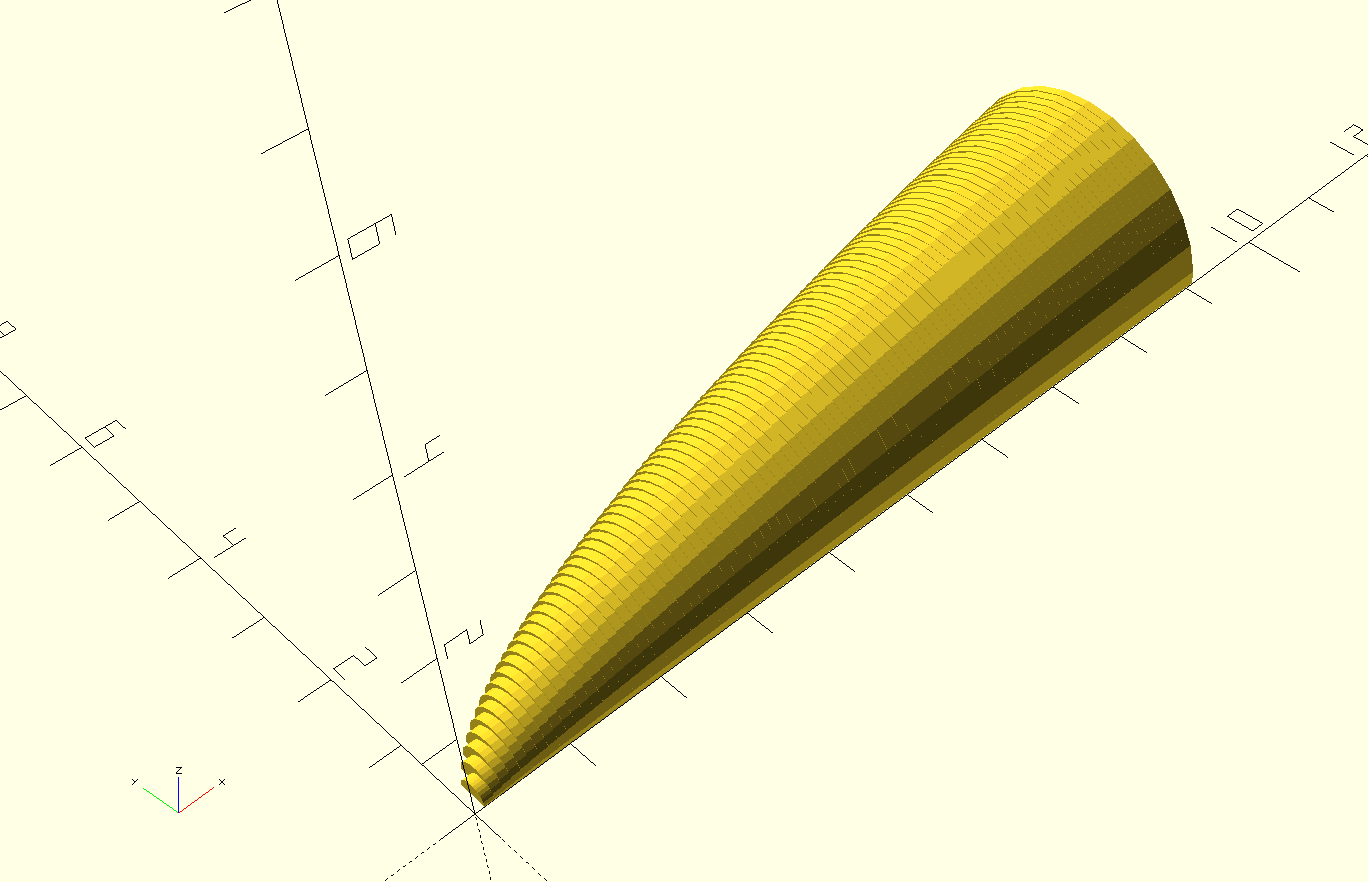
\includegraphics[width=.9\linewidth]{KBe21math401retCrossSectionSolidFinalB.png}
\end{center}

\begin{center}
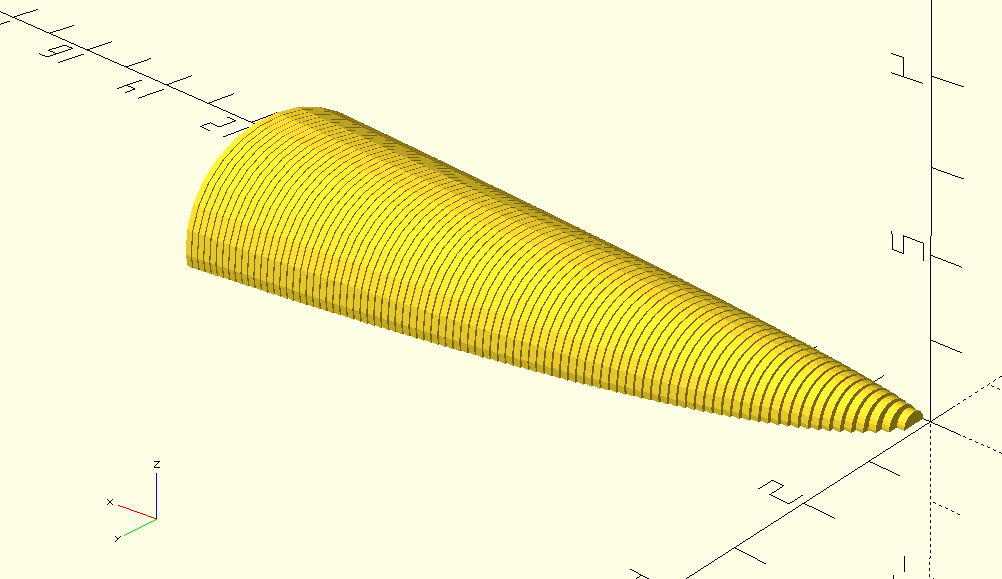
\includegraphics[width=.9\linewidth]{KBe21math401retCrossSectionSolidFinalB2.png}
\end{center}

\begin{center}
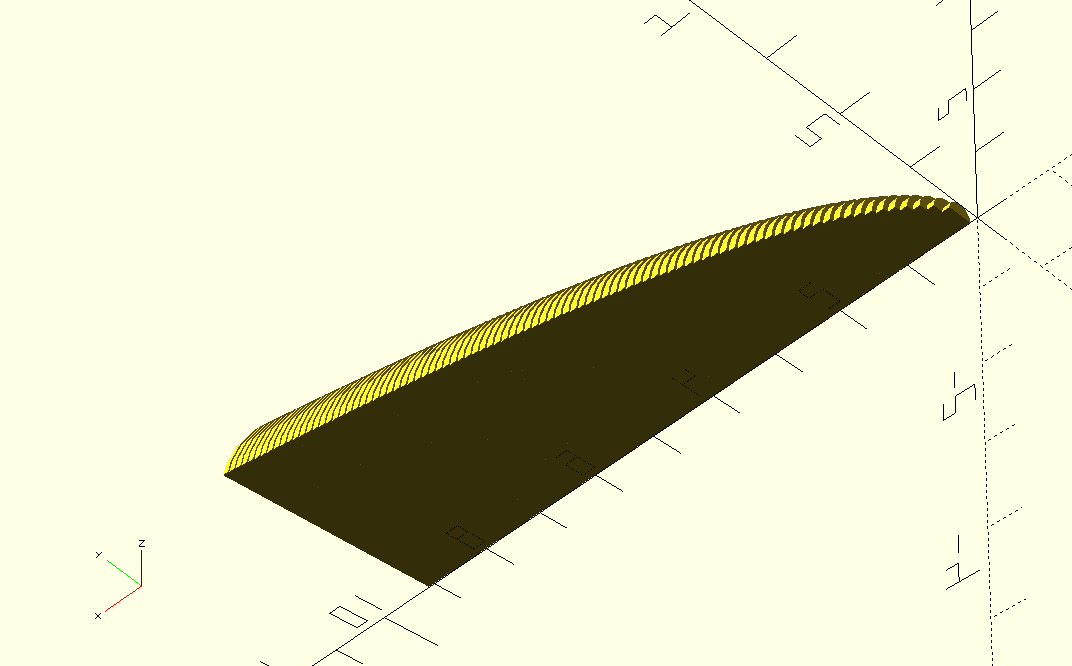
\includegraphics[width=.9\linewidth]{KBe21math401retCrossSectionSolidFinalB3.png}
\end{center}
\end{document}
